\documentclass[]{article}
\usepackage{amsmath, amsfonts}
\usepackage{enumitem}
\usepackage{fancyhdr}
\usepackage{geometry}
\usepackage{cancel}
\usepackage{graphicx}
\usepackage{color}
\usepackage{soul}
\usepackage{multirow}
\usepackage{float}
\usepackage{pgfplots}	% To draw charts directly in Latex
\usepackage{marvosym}	% For lightning symbol to denote contradiction
\usepackage{cleveref}	% For clever referencing :)
\usepackage{nameref}	% For referencing to the section name, not number
\usepackage{slashbox}

%TikZ package for drawing:
\usepackage{tikz}
%For calculation of coordinates:
\usetikzlibrary{calc}
\usetikzlibrary{positioning}

\geometry{a4paper, left=20mm, top=20mm, bottom = 20mm, headheight=20mm}

\sloppy
\definecolor{lightgray}{gray}{0.5}
\setlength{\parindent}{0pt}

\renewcommand{\arraystretch}{1.3}

\begin{document}

\textbf{Problem Set 1, Exercise 7 (from 2009 exam)}

Nurfatima Jandarova

\today
\\

Define the set of actions available to players 1 and 2 $\{P, N\}$, where $P$ stands for 'Pass' and $N$ stands for 'Not pass'. Denote the set of actions available to the player 3 $\{P1, P2, P0\}$, where $P1$ stands for 'Punish player 1', $P2$ stands for 'Punish player 2' and $P0$ stands for 'Punish no one'. Then, the game in extensive form is:
\begin{figure}[h]
	\begin{center}
		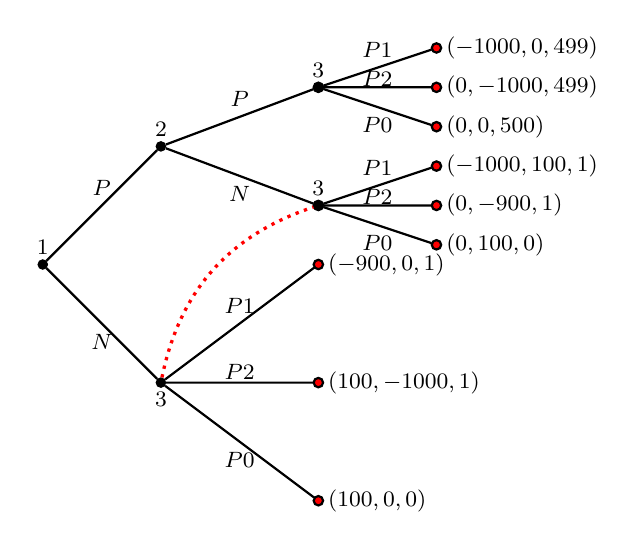
\begin{tikzpicture}
		[
		grow =right,
		font=\footnotesize,
		edge from parent/.style={draw,thick}
		]
		
		% Two node styles: solid and hollow
		\tikzstyle{solid node}=[circle,draw,inner sep=1.2,fill=black];
		\tikzstyle{end node}=[circle,draw,inner sep=1.2,fill=red];
		\tikzstyle{hollow node}=[circle,draw,inner sep=1.2];
		
		% Specify spacing for each level of the tree
		\tikzstyle{level 1}=[level distance=15mm,sibling distance=30mm]
		\tikzstyle{level 2}=[level distance=20mm,sibling distance=15mm]
		\tikzstyle{level 3}=[level distance=15mm,sibling distance=5mm]
		% The Tree
		\node(0)[solid node]{}
				% Player 1, Not pass
		child{node[solid node]{} 
			child{node[end node]{} edge from parent node[below]{$P0$}}
			child{node[end node]{} edge from parent node[yshift=4]{$P2$}}
			child{node[end node]{} edge from parent node[above]{$P1$}}
		edge from parent node[below]{$N$}}
		% Player 1, Pass
		child{node[solid node]{} 
			child{node[solid node]{} 
				child{node[end node]{} edge from parent node[below]{$P0$}}
				child{node[end node]{} edge from parent node[yshift=3]{$P2$}}
				child{node[end node]{} edge from parent node[above]{$P1$}}
				edge from parent node[below]{$N$}}
			child{node[solid node]{}
				child{node[end node]{} edge from parent node[below]{$P0$}}
				child{node[end node]{} edge from parent node[yshift=3]{$P2$}}
				child{node[end node]{} edge from parent node[above]{$P1$}}
				edge from parent node[above]{$P$}}
			edge from parent node[above]{$P$}}
		;
		% Information sets
		\draw[dotted, bend left, draw=red, very thick](0-1)to(0-2-1);
		
		% Players
		% player 1
		\node[above]at(0){1};
		% player 2
		\node[above]at(0-2){2};
		% player 3
		\node[below]at(0-1){3};
		\foreach \y in {1, 2} \node[above]at(0-2-\y){3};
		
		% Specifying payoffs
		\node[right]at(0-1-1){$(100, 0, 0)$};
		\node[right]at(0-1-2){$(100, -1000, 1)$};
		\node[right]at(0-1-3){$(-900, 0, 1)$};
		\node[right]at(0-2-1-1){$(0, 100, 0)$};
		\node[right]at(0-2-1-2){$(0, -900, 1)$};
		\node[right]at(0-2-1-3){$(-1000, 100, 1)$};
		\node[right]at(0-2-2-1){$(0, 0, 500)$};
		\node[right]at(0-2-2-2){$(0, -1000, 499)$};
		\node[right]at(0-2-2-3){$(-1000, 0, 499)$};
		
		\end{tikzpicture}
	\end{center}
%	\caption{A centipede game in extensive form}
%	\label{fig:ex1ext}
\end{figure}

There are three players, i.e., $N = \{1, 2, 3\}$ and their strategy spaces could be defined as
\begin{equation}
	\begin{split}
		S_1& = \{P, N\} \\ \nonumber
		S_2& = \{P, N\} \\
		S_3& = \{P1, P2, P0\}^2 = \{(P1, P1), (P1, P2), (P1, P0), (P2, P1), (P2, P2), (P2, P0), (P0, P1), (P0, P2), (P0, P0)\}
	\end{split}
\end{equation}
We could also define the profit functions
\begin{equation}
	\begin{split}
		\pi_1: S_1\times S_2 \times S_3 \to \{-1000, -900, 0, 100\} \\ \nonumber
		\pi_2: S_2\times S_1 \times S_3 \to \{-1000, -900, 0, 100\} \\
		\pi_3: S_3\times S_1 \times s_2 \to \{0, 1, 499, 500\}
	\end{split}
\end{equation}
or in table form
\begin{table}[h]
	\centering
	\begin{minipage}{0.5\linewidth}
		\centering
		Player 1 plays $P$\\
		\begin{tabular}{c|cc}
			\backslashbox{3}{2} & P & N \\ \hline
			(P1, P1) & (-1000, 0, 499) & (-1000, 100, 1) \\
			(P1, P2) & (-1000, 0, 499) & (0, -900, 1) \\
			(P1, P0) & (-1000, 0, 499) & (0, 100, 0) \\
			(P2, P1) & (0, -1000, 499) & (-1000, 100, 1) \\
			(P2, P2) & (0, -1000, 499) & (0, -900, 1) \\
			(P2, P0) & (0, -1000, 499) & (0, 100, 0) \\
			(P0, P1) & (0, 0, 500) & (-1000, 100, 1) \\
			(P0, P2) & (0, 0, 500) & (0, -900, 1) \\
			(P0, P0) & (0, 0, 500) & (0, 100, 0)
		\end{tabular}
	\end{minipage}%
	\begin{minipage}{0.5\linewidth}
		\centering
		Player 1 plays $N$\\
		\begin{tabular}{c|cc}
			\backslashbox{3}{2} & P & N \\ \hline
			(P1, P1) & (-900, 0, 1) & (-900, 0, 1) \\
			(P1, P2) & (100, -1000, 1) & (100, -1000, 1) \\
			(P1, P0) & (100, 0, 0) & (100, 0, 0) \\
			(P2, P1) & (-900, 0, 1) & (-900, 0, 1) \\
			(P2, P2) & (100, -1000, 1) & (100, -1000, 1) \\
			(P2, P0) & (100, 0, 0) & (100, 0, 0) \\
			(P0, P1) & (-900, 0, 1) & (-900, 0, 1) \\
			(P0, P2) & (100, -1000, 1) & (100, -1000, 1) \\
			(P0, P0) & (100, 0, 0) & (100, 0, 0)
		\end{tabular}
	\end{minipage}
\end{table}

\end{document}
